% XCircuit output "blockpa.tex" for LaTeX input from blockpa.ps
\def\putbox#1#2#3#4{\makebox[0in][l]{\makebox[#1][l]{}\raisebox{\baselineskip}[0in][0in]{\raisebox{#2}[0in][0in]{\scalebox{#3}{#4}}}}}
\def\rightbox#1{\makebox[0in][r]{#1}}
\def\centbox#1{\makebox[0in]{#1}}
\def\topbox#1{\raisebox{-0.60\baselineskip}[0in][0in]{#1}}
\def\midbox#1{\raisebox{-0.20\baselineskip}[0in][0in]{#1}}
   \scalebox{1}{
   \normalsize
   \parbox{6.88021in}{
   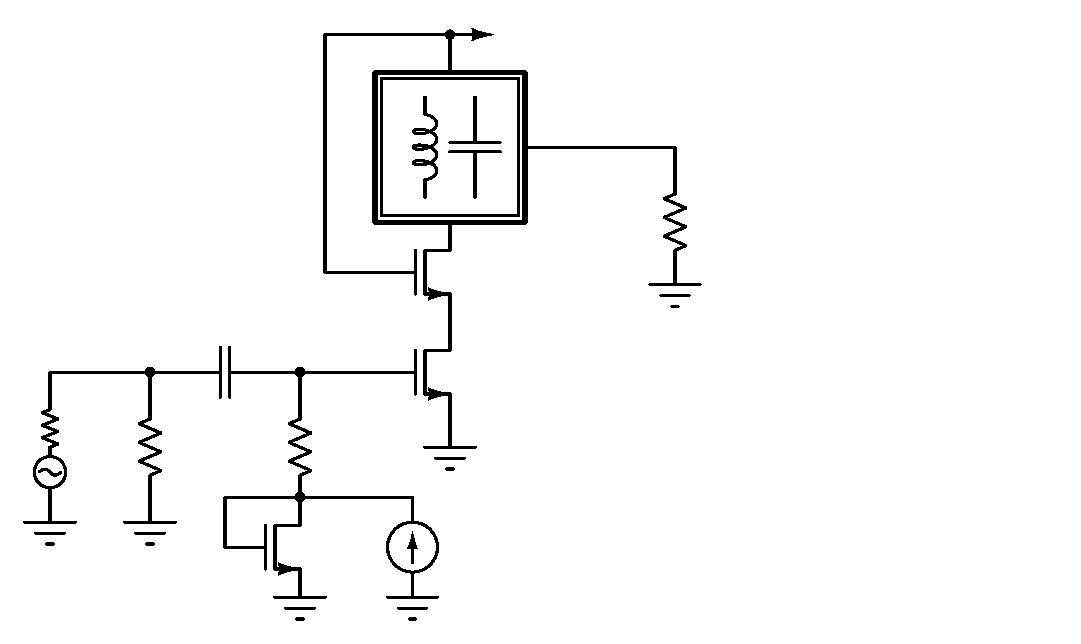
\includegraphics[scale=1]{blockpa}\\
   % translate x=608 y=476 scale 0.38
   \putbox{2.91in}{1.70in}{1.20}{\midbox{}}%
   \putbox{2.91in}{1.37in}{1.20}{}%
   \putbox{2.91in}{2.37in}{1.20}{\midbox{}}%
   \putbox{2.91in}{2.04in}{1.20}{}%
   \putbox{3.22in}{3.95in}{1.20}{\midbox{$V_\mr{DD}=1.2~\mr{ili}~2.5~\mr{V}$}}%
   \putbox{4.50in}{2.64in}{1.20}{$50~\Omega$}%
   \putbox{0.36in}{1.04in}{1.20}{\midbox{$P_\mr{in}$}}%
   \putbox{0.31in}{1.29in}{1.20}{\midbox{$10~\Omega$}}%
   \putbox{1.00in}{1.14in}{1.20}{$10~\Omega$}%
   \putbox{2.00in}{1.14in}{1.20}{$10~\mr{k}\Omega$}%
   \putbox{2.89in}{1.70in}{1.20}{\midbox{$m\frac{W}{L}$}}%
   \putbox{1.91in}{0.54in}{1.20}{\midbox{}}%
   \putbox{1.91in}{0.20in}{1.20}{}%
   \putbox{1.89in}{0.54in}{1.20}{\midbox{$\frac{W}{L}$}}%
   \putbox{2.81in}{0.54in}{1.20}{\midbox{$W\cdot I_D/W$}}%
   \putbox{1.39in}{1.95in}{1.20}{\centbox{$1~\mr{nF}$}}%
   \putbox{3.06in}{0.29in}{1.20}{\midbox{$I_D/W=100-300~\mu\mr{A}/\mu\mr{m}$}}%
   } % close 'parbox'
   } % close 'scalebox'
   \vspace{-\baselineskip} % this is not necessary, but looks better
